\documentclass{article}
\usepackage[utf8]{inputenc}

\usepackage{url}
\usepackage{float}
\usepackage{natbib}
\usepackage{authblk}
\usepackage{graphicx}
\usepackage{listings}
\usepackage{fullpage}
\usepackage{hyperref}
\hypersetup{
    colorlinks=true,
    linkcolor=blue,
    filecolor=magenta,      
    urlcolor=cyan,
}
\title{Small Bot Motor Control Shield Hardware Manual}
\author[1]{Matt Ruffner}
\author[1]{Damien Lawhorn}
\author[1]{Josh Ashley}
\affil[1]{University of Kentucky}
\date{July 10, 2020}
\setcounter{Maxaffil}{0}
\renewcommand\Affilfont{\itshape\small}
\begin{document}

\maketitle
\tableofcontents
%\newpage
\listoffigures
\listoftables
%\newpage

\section{Introduction}
This document contains information relevant to the design of the Small Bot Motor Control Shield (SBMCS). The SBMCS is being developed by the Kentcuky Organization of Robotics and Automation (KORA) student led club at the University of Kentucky.

\appendix
\label{sec:appa}

\section{SBMCS Arduino Pin Assignment}
\begin{figure}[H]
    \centering
    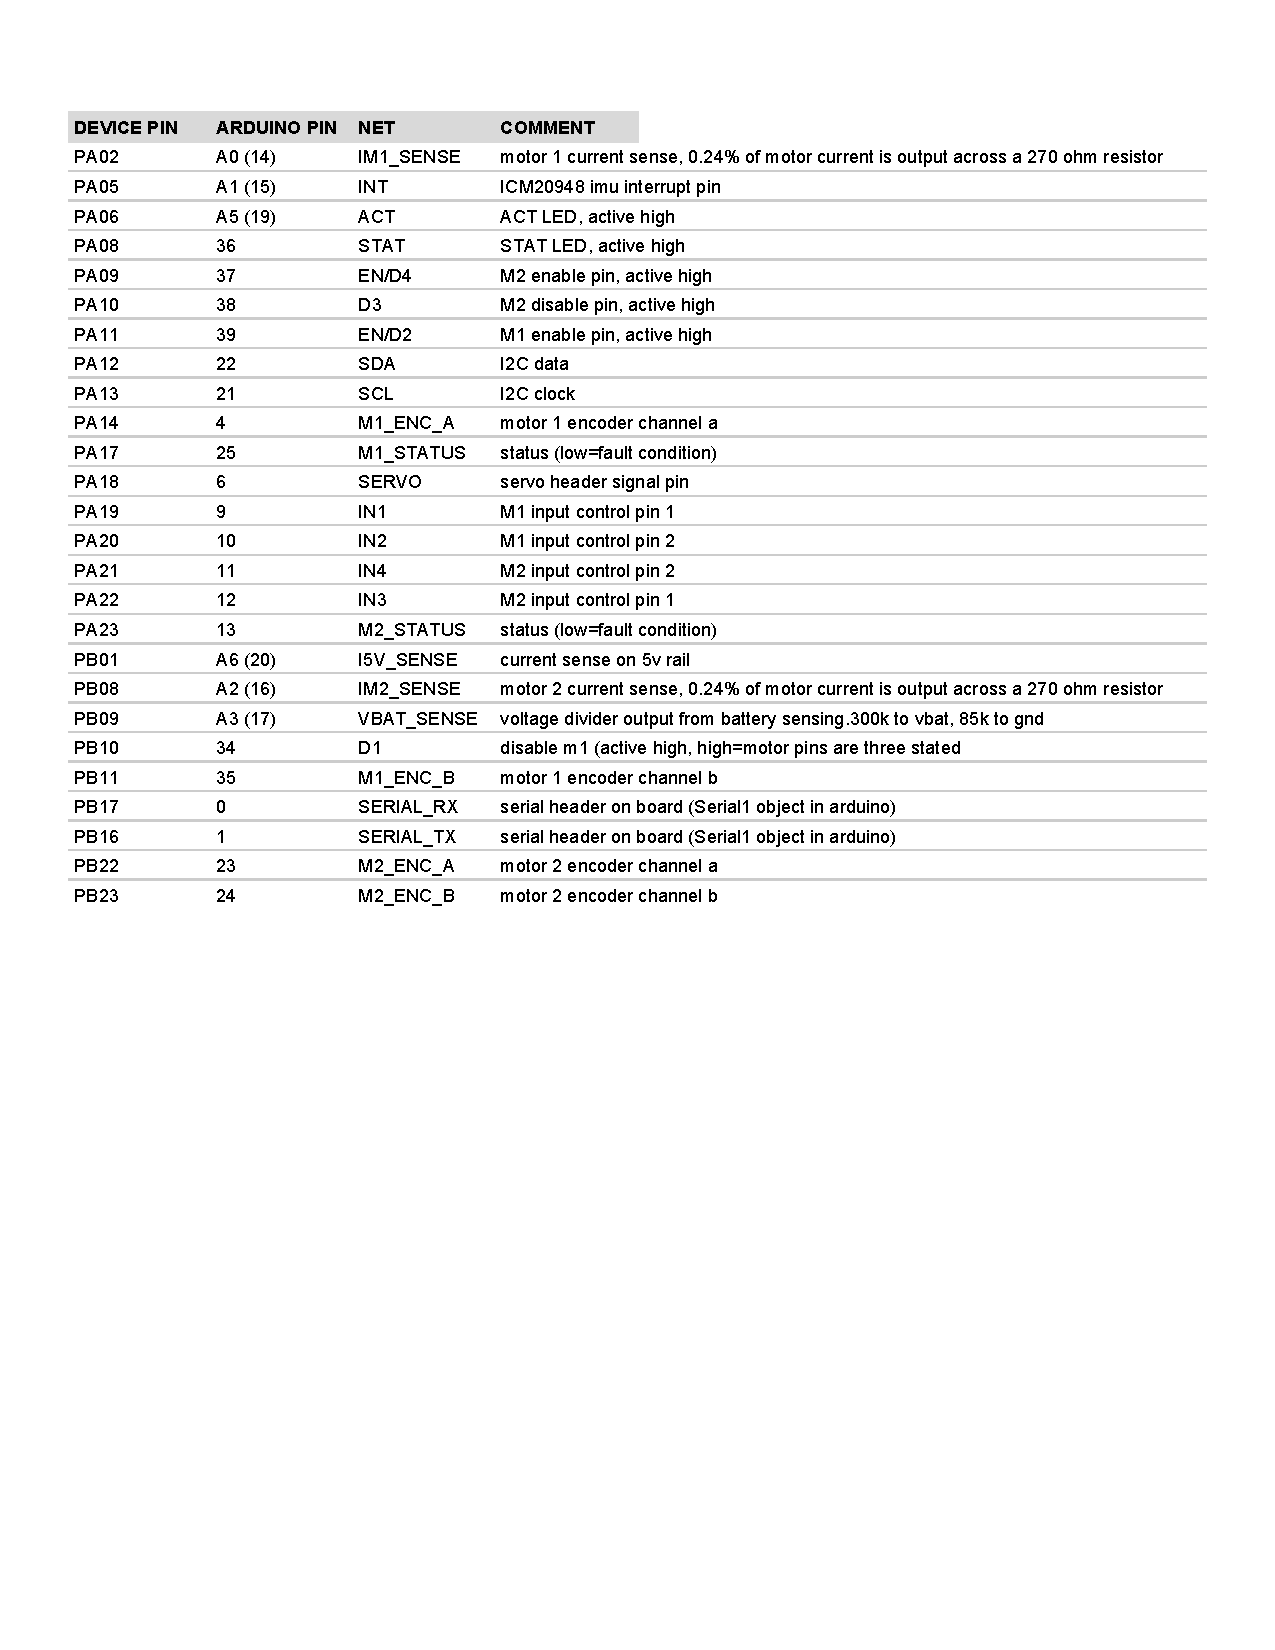
\includegraphics[width=\textwidth]{sbmcs-arduino-pinmap.pdf}
    \label{fig:sbmcs-arduino-pinmap}
\end{figure}



\section{Feather M4 Arduino Reference}
Courtesy of Adafruit Industries
\begin{figure}[H]
    \centering
    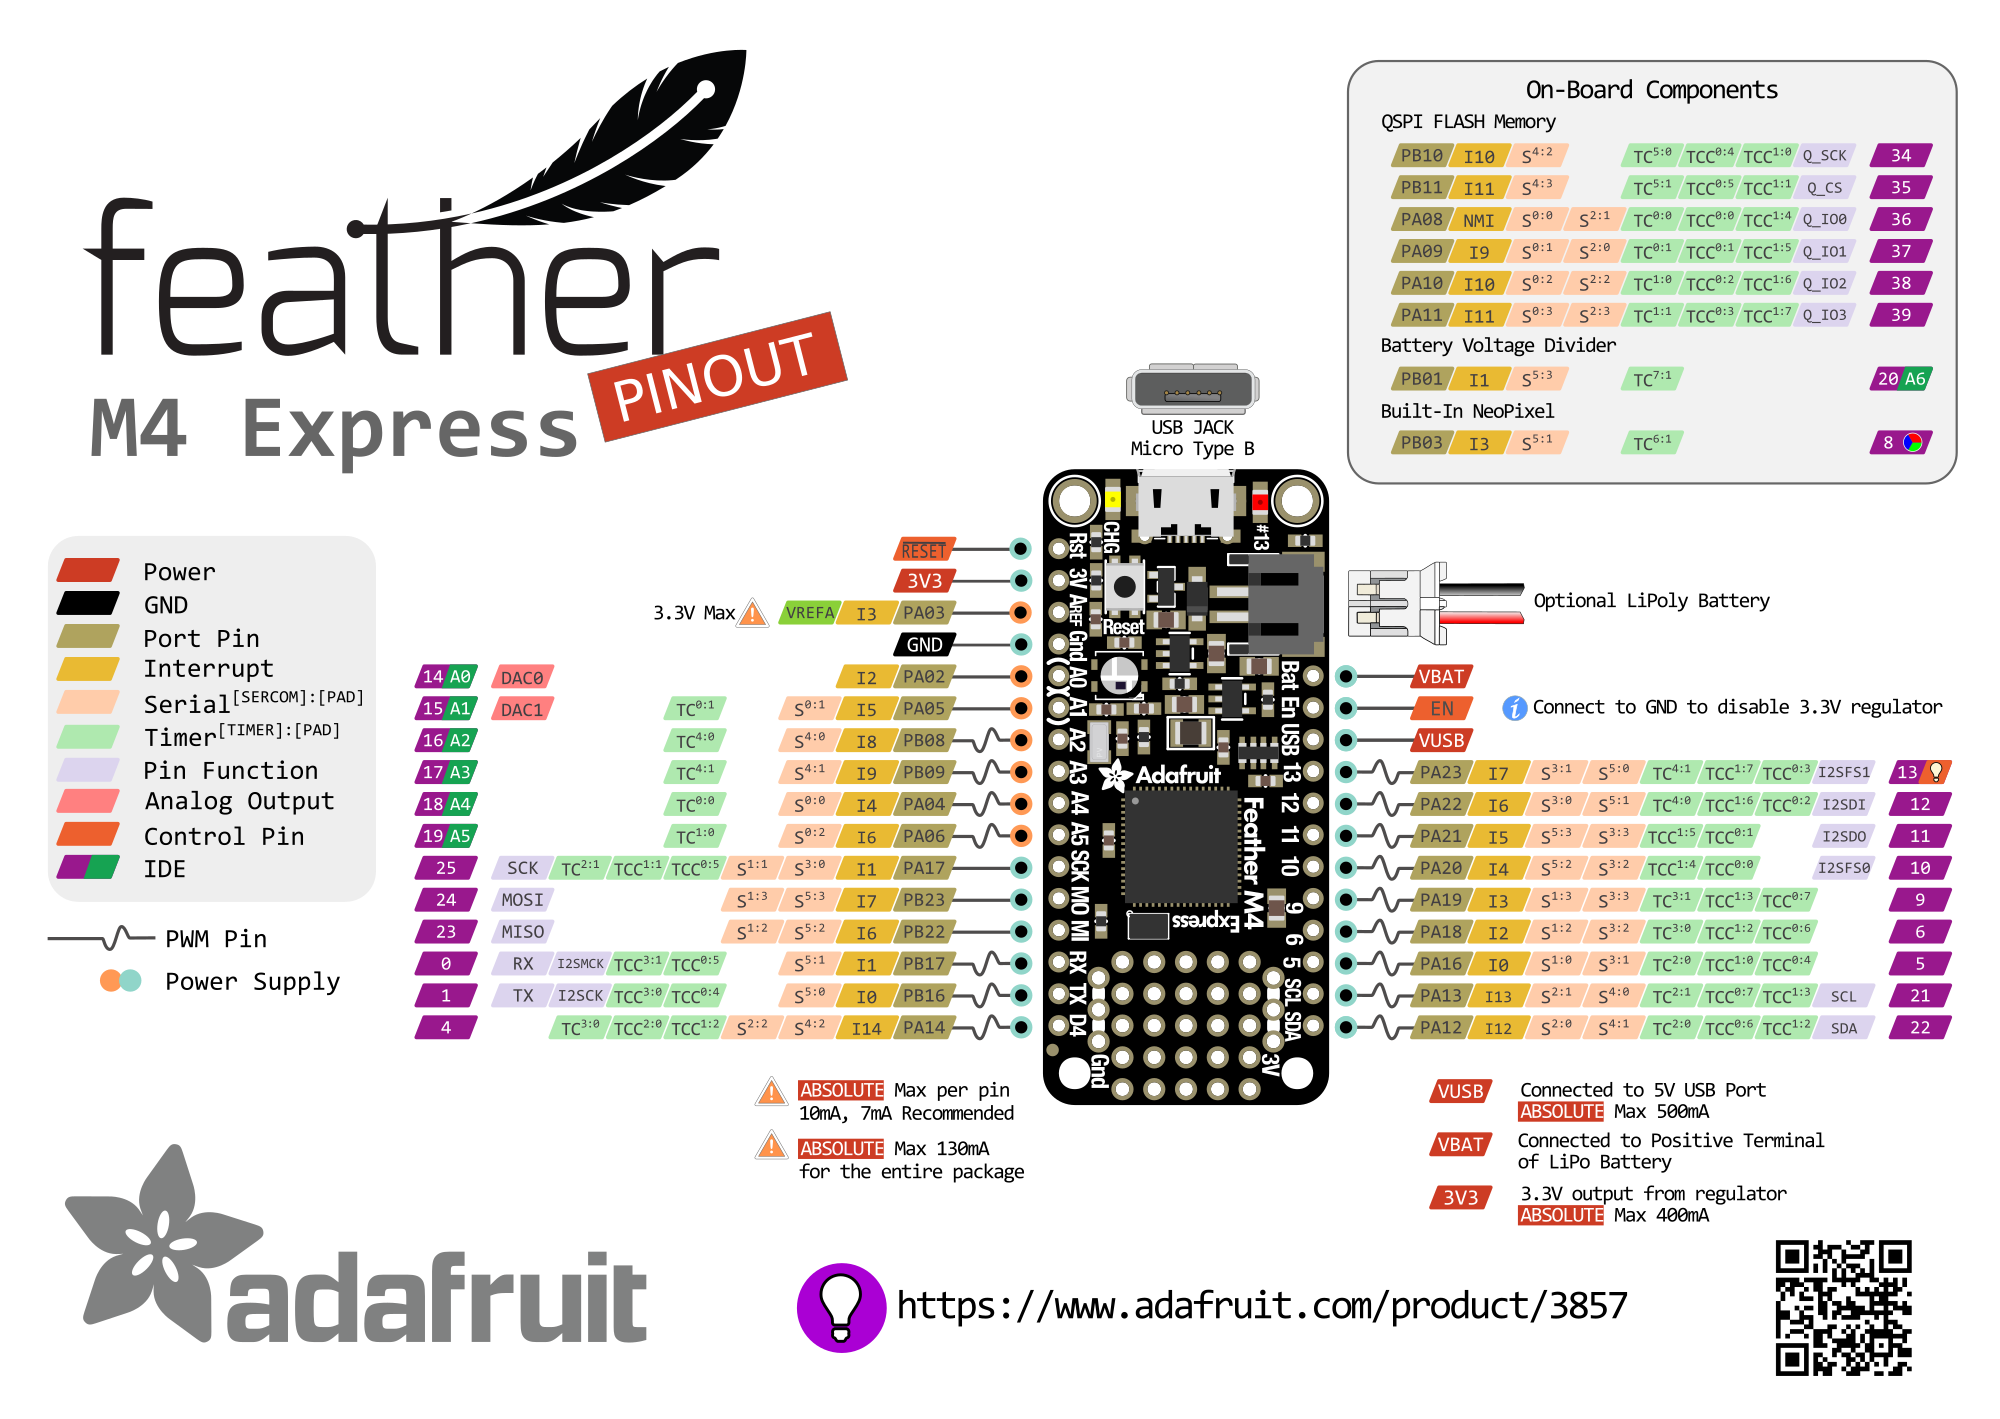
\includegraphics[width=\textwidth]{images/arduino_compatibles_Feather_M4_Page.png}
    \label{fig:m4-pinout}
\end{figure}

\end{document}
